%%%%%%%%%%%%%%%%%%%%%%%%%%%%%%%%%%%%%%%%%
% University Assignment Title Page
% LaTeX Template
% Version 1.0 (27/12/12)
%
% This template has been downloaded from:
% http://www.LaTeXTemplates.com
%
% Original author:
% WikiBooks (http://en.wikibooks.org/wiki/LaTeX/Title_Creation)
%
% License:
% CC BY-NC-SA 3.0 (http://creativecommons.org/licenses/by-nc-sa/3.0/)
%
% Instructions for using this template:
% This title page is capable of being compiled as is. This is not useful for
% including it in another document. To do this, you have two options:
%
% 1) Copy/paste everything between \begin{document} and \end{document}
% starting at \begin{titlepage} and paste this into another LaTeX file where you
% want your title page.
% OR
% 2) Remove everything outside the \begin{titlepage} and \end{titlepage} and
% move this file to the same directory as the LaTeX file you wish to add it to.
% Then add \input{./title_page_1.tex} to your LaTeX file where you want your
% title page.
%
%%%%%%%%%%%%%%%%%%%%%%%%%%%%%%%%%%%%%%%%%
%\title{Title page with logo}
%----------------------------------------------------------------------------------------
%   PACKAGES AND OTHER DOCUMENT CONFIGURATIONS
%----------------------------------------------------------------------------------------

\documentclass[12pt]{article}
\usepackage[english]{babel}

\usepackage{float}
% \usepackage{subfig}
\usepackage{wrapfig}
\usepackage[utf8]{inputenc}
\usepackage[top=1in, bottom=1in, left=1.25in, right=1.25in]{geometry}
\usepackage{amsmath}
\usepackage[toc,page]{appendix}
\usepackage{graphicx}
\usepackage{listings}
\usepackage{framed}
\usepackage{footmisc}
\usepackage{amssymb}
\usepackage{hyperref}
\usepackage{cleveref}
\usepackage{listings}
\usepackage{listingsutf8}
\usepackage{ucs}
\usepackage[affil-it]{authblk}
\graphicspath{ {figures/}}
\usepackage[colorinlistoftodos]{todonotes}
\lstset{numbers=none,
numberstyle=\tiny,
keywordstyle=\color{blue!70}, commentstyle=\color{red!50!green!50!blue!50},
frame=single,inputencoding=utf8x,
rulesepcolor=\color{red!20!green!20!blue!20},
breaklines=true,basicstyle=\scriptsize
}



\begin{document}

\begin{titlepage}

\newcommand{\HRule}{\rule{\linewidth}{0.5mm}} % Defines a new command for the horizontal lines, change thickness here

\center % Center everything on the page

%----------------------------------------------------------------------------------------
%   HEADING SECTIONS
%----------------------------------------------------------------------------------------

\textsc{\LARGE University of California, Davis}\\[1cm] % Name of your university/college
\textsc{\Large Department of Land, Air and Water}\\[0.5cm] % Major heading such as course name
% \textsc{\large Minor Heading}\\[0.5cm] % Minor heading such as course title

%----------------------------------------------------------------------------------------
%   TITLE SECTION
%----------------------------------------------------------------------------------------

\HRule \\[0.4cm]
{ \huge \bfseries Field Data-logger 1.0}\\[0.4cm] % Title of your document
\HRule \\[1cm]

%----------------------------------------------------------------------------------------
%   AUTHOR SECTION
%----------------------------------------------------------------------------------------

% \begin{minipage}{0.4\textwidth}
% \begin{flushleft} \large
% \emph{Members:}\\
% Hengjiu \textsc{Kang}   \\ % Your name  \\
% \end{flushleft}
% \end{minipage}
% ~
% \begin{minipage}{0.4\textwidth}
% \begin{flushright} \large
% \emph{Supervisor:} \\
% Dr. Andre \textsc{Knoesen} % Supervisor's Name
% \end{flushright}
% \end{minipage}\\[2cm]

% If you don't want a supervisor, uncomment the two lines below and remove the section above
\Large \emph{Author:}\\
Hengjiu \textsc{Kang}\\[3cm] % Your name

%----------------------------------------------------------------------------------------
%   DATE SECTION
%----------------------------------------------------------------------------------------

{\large \today}\\[1.5cm] % Date, change the \today to a set date if you want to be precise

%----------------------------------------------------------------------------------------
%   LOGO SECTION
%----------------------------------------------------------------------------------------

% 
\includegraphics[scale=0.5]{uc-davis.png}\\[1cm] % Include a department/university logo - this will require the graphicx package

%----------------------------------------------------------------------------------------

\vfill % Fill the rest of the page with whitespace

\end{titlepage}

\author{Hengjiu Kang%
  \thanks{Electronic address: \texttt{hjkang@ucdavis.edu}}}
\affil{Department of Electrical and Computer Engineering, University of California, Davis}


\title{Field Data-Loger 1.0}
\maketitle

\newpage
\begin{figure}[H]
\centering
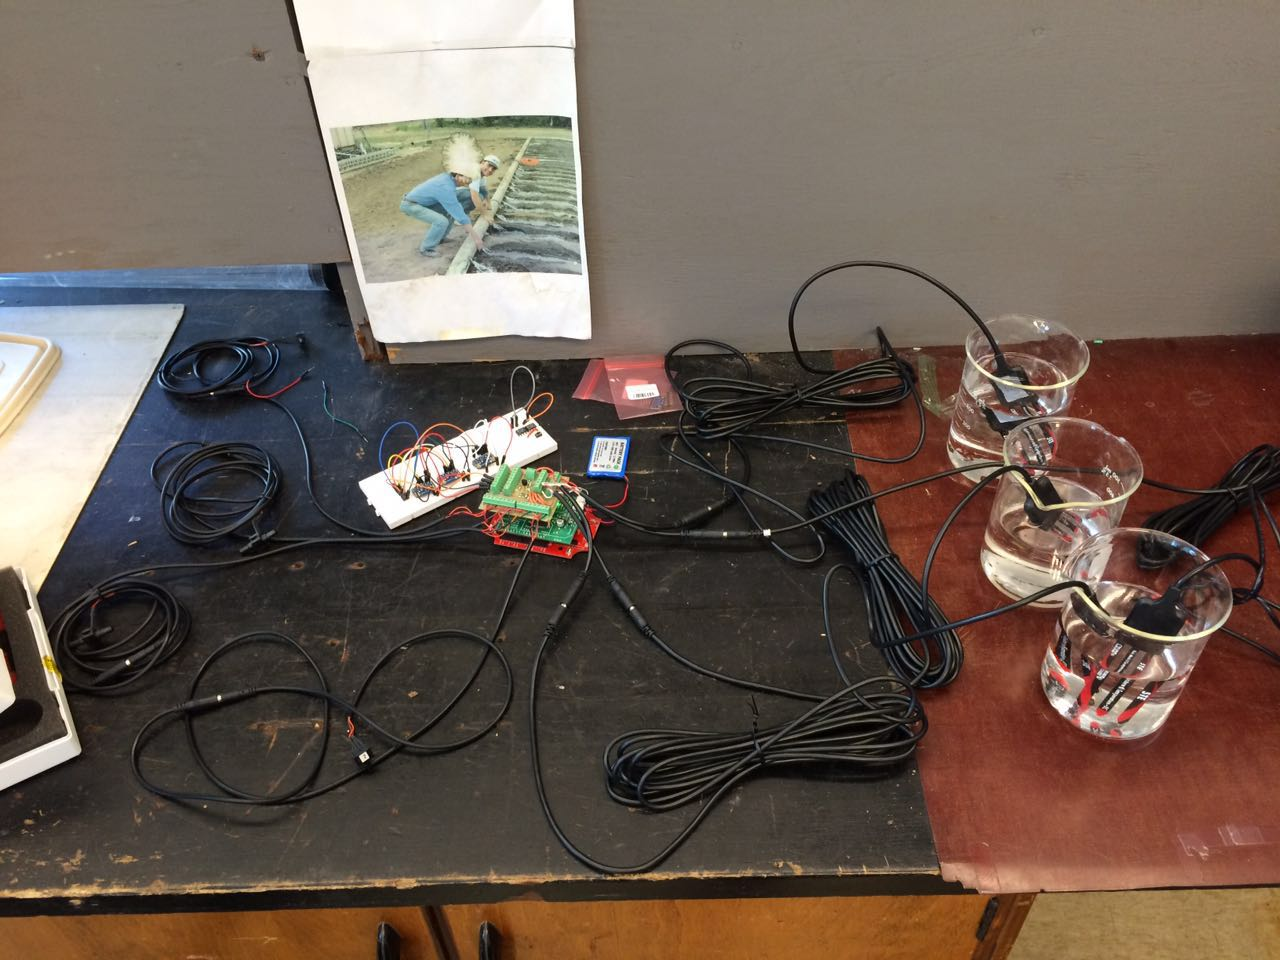
\includegraphics[width=\textwidth]{overall.jpg}
\caption{\emph{Overall view of field Data-logger}}
\end{figure}

\newpage
\tableofcontents \newpage
\listoffigures  \newpage

\newpage

\section{Overview}
    This Field Data-logger is a new hardware based on Atmega328 chip which fuses multiple type of sensors from different brands. It can collect data in programmable period of time, and thanks to low power design, this Field Data-logger can last for very long time when solar panel is installed.

\section{Features}
    \begin{itemize}
    \item 8 16-bit single ended or 4 16-bit differential ADC inputs
    \item 4 $I^{2}C$ connection ports
    \item 4 Read only sensors inputs
    \item Programmable wake up RTC
    \item Solar panel
    \item On-board SD card
    \item XBee network (Will be available in the next version)
    \end{itemize}


\newpage
\section{Hardware Design}
  \subsection{Absolut values}
    \label{absValue}
\begin{table}[H]
\centering
\begin{tabular}{|l|l|l|l|l|l|l|}
Parameter               & Sym   & Min  & Typ          & Max & Unit & Conditions \\
External Battery        & Vbat  & 3.2  & 3.8          & 4.2 & V    &            \\
Digital Pin HIGH        & Vhigh & 3.3  & 3.3          &     & V    &            \\
Digital Pin Low         & Vlow  & 0    & 0            & 0.2 & V    &            \\
Voltage Boost Output    & 5V    & 5.0  & 5.2          & 5.3 & V    &            \\
ADC Sample rate         & tADC  &      & 800          &     & sps  &            \\
Boot time               & tBoot &      & 0.5          &     & s    &            \\
5TE sensor cooling time &       &      & 2            &     & s    &            \\
ADC minimum input       &       & -0.5 &              &     & V    &            \\
ADC maximum input       &       &      &              & 5.5 & V    &            \\
Default sleep period    &       &      & 60           &     & min  &            \\
System sleep current    &       &      & \textless100 &     & uA   &            \\
System active current   &       &      &              & 45  &      &           
\end{tabular}
\end{table}





  \subsection{Electrical Systems}
  This field data-logger is designed in stack strategy to reach more compact size and more flexible connectivity. On the bottom is the main controller, middle shield is functionality shield, which has all the functional peripheral circuits on it, including external high precision ADC chip, power regulation circuit and level shifting circuit. Also, it has a 20-pin header pins to connect to the top shield, connection shield. Connection shield bears all the terminal connectors and simple protection circuits.

    \subsubsection{Controller board}
    \begin{figure}[ht]
    \centering
    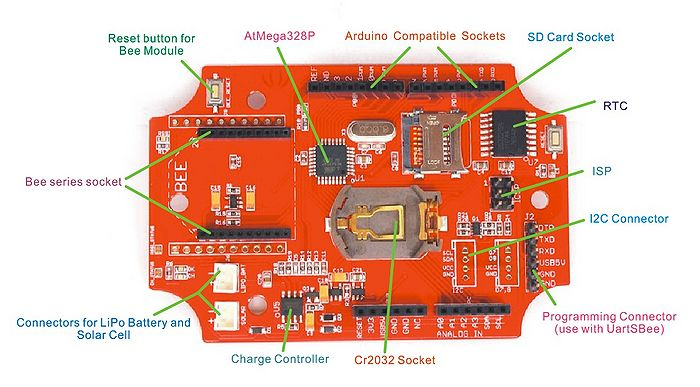
\includegraphics[width=0.9\textwidth]{Stalker.jpg}
    \caption{\label{fig:Seeeduino Stalker}Seeeduino Stalker v2.3}
    \end{figure}
  Arduino Based controller Seeeduino Stalker v2.3 has been used as main controller. This controller is fully compatible with Arduino structure, and also it is able to connect to external Li-ion battery and a solar panel. According to our test, in UC Davis campus area, sun light is able to keep data-logger always on. 

    \subsubsection{Functionality board}
    \begin{figure}[H]
    \centering
    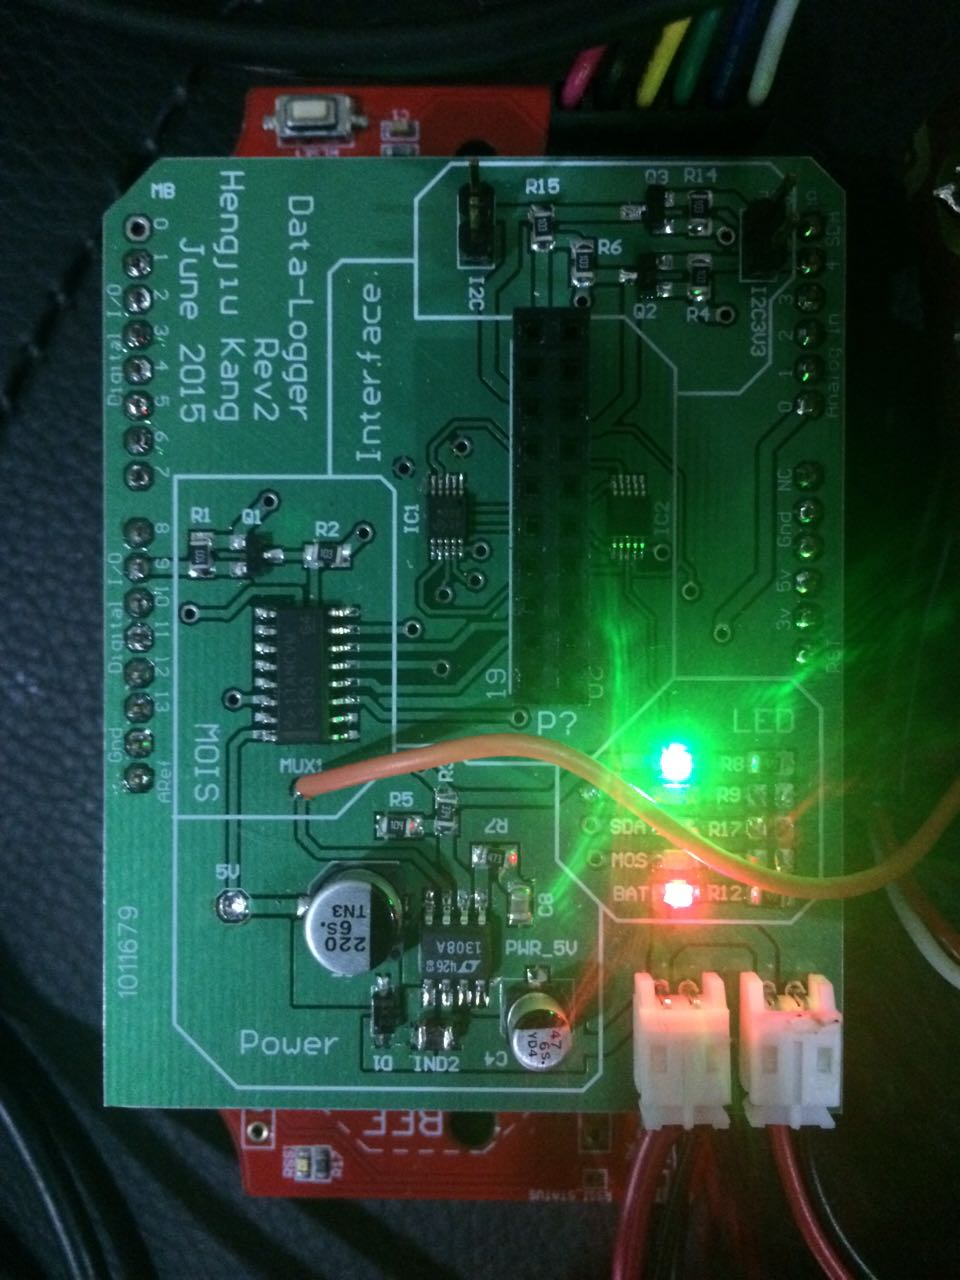
\includegraphics[width=0.9\textwidth]{func_board_top.jpg}
    \caption{\label{fig:Func Board}Functionality Board Top view}
    \end{figure}
    Functionality board is consisted of five functional blocks.
    \begin{enumerate}
    \item $I^{2}C$ Level shifting blocks  \\
      Because all the sensors are powered by 5V power source, so there is a 2-way level shifting circuit here to convert $I^{2}C$ connection. Refering to \hyperref[i2c Design]{\textbf{\textit{I2C Design}}} for more information.
    \item Interface blocks\\
      A 20-pin housing to connect to connection board.
    \item MOIS blocks \\
      MOIS refers to 'Moisture sensor'. Default moisture sensor this data-logger uses is 5TE moisture sensor from decagon company, which uses 1-wire communication protocal, and there is a MUX chip let the board read at most 4 5TE sensors. Refering to \hyperref[read-only Design]{\textbf{\textit{Read-only Port}}} for more information.
    \item Power blocks  \\
      Power block is circuit to convert battery voltage to 5V standard voltage powering all the devices. Refering to \hyperref[power block]{\textbf{\textit{On-board power}}} for more information.
    \item LED blocks    \\
      There are also five LEDs in this block for debugging purpose.
    \end{enumerate}

    \subsubsection{Connectivity board}
    \begin{figure}[H]
    \centering
    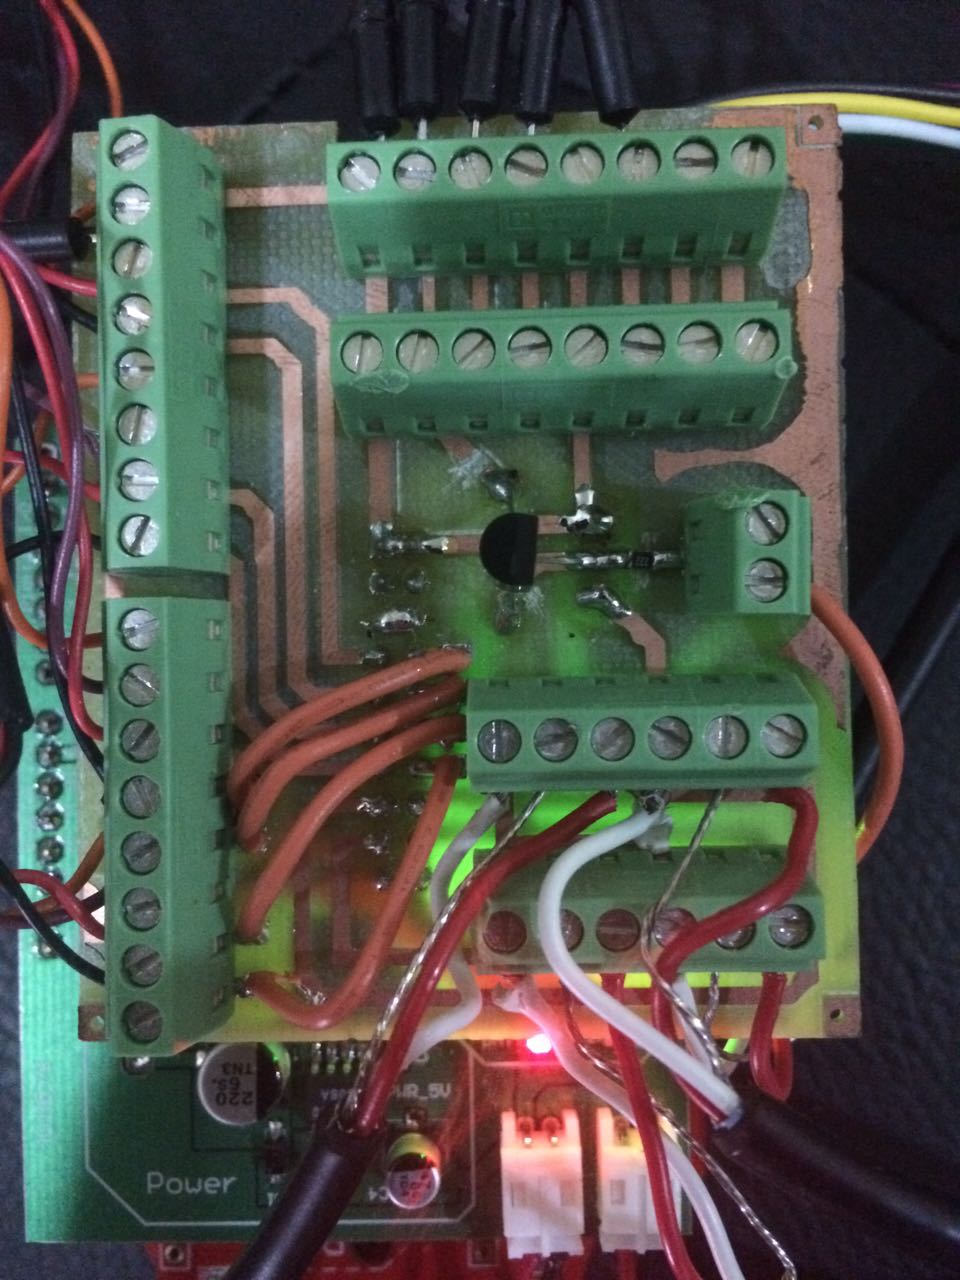
\includegraphics[width=0.9\textwidth]{con_board_top.jpg}
    \caption{\label{fig:Con Board}Connectivity Board Top view}
    \end{figure}

    Connectivity board has almost the same dimension of the functionality board and controller board, which is good to fit in the box. In order to increase the reliability of connection, 350 series terminal connector from Phoenix was chosen to make the job done. All the connections are following the wire order :\\
    \begin{itemize}
    \item VCC
    \item GND
    \item connection 1 (SCL/ADC+)
    \item connection 2 (SDA/ADC-)
    \item etc..
    \end{itemize}

  
  \subsection{Power}
  \subsubsection{External power supply}
    \begin{figure}[ht]
    \centering
    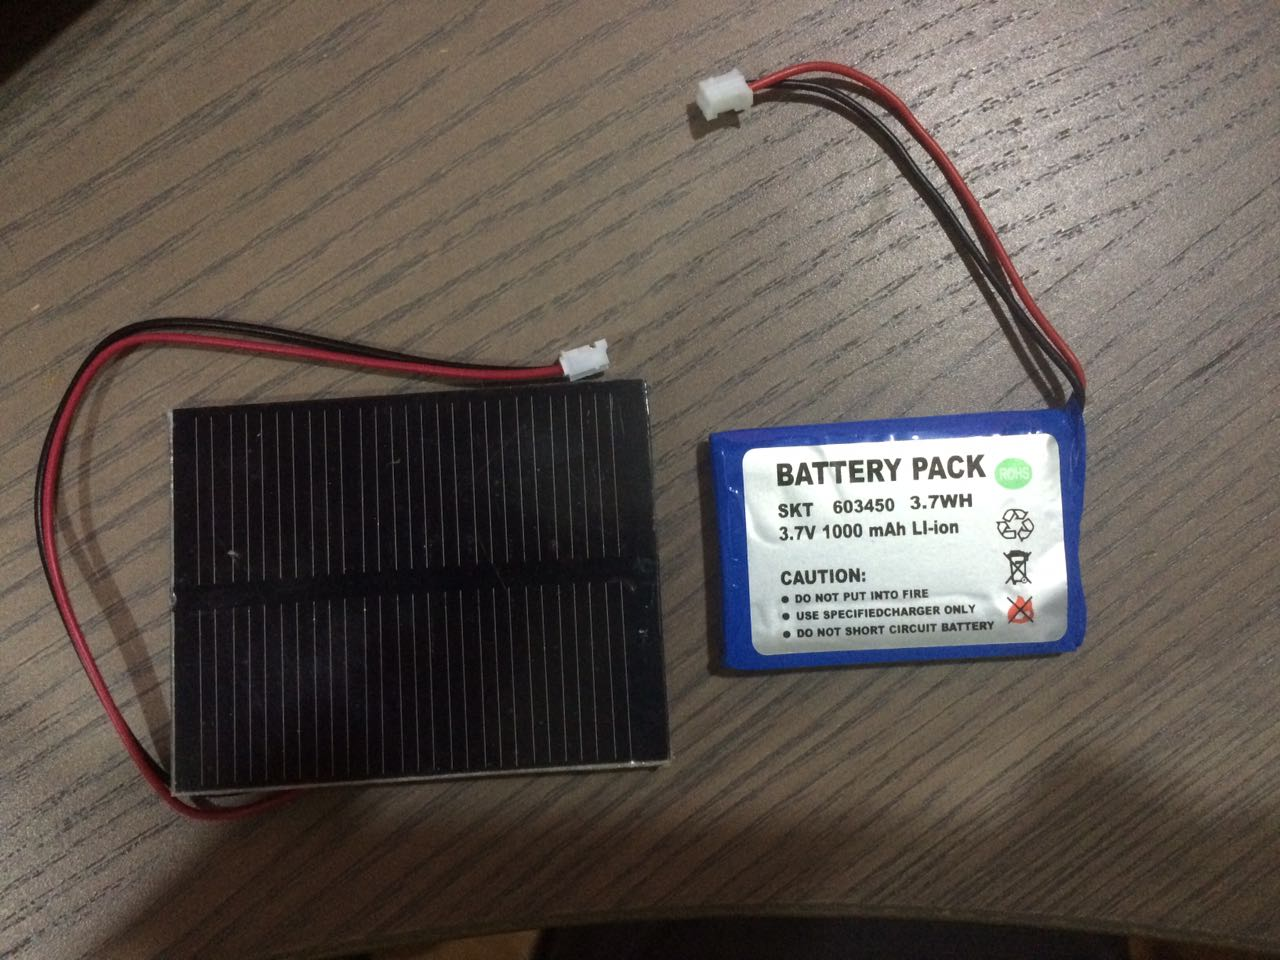
\includegraphics[width=0.9\textwidth]{battery_solar.jpg}
    \caption{\label{fig:Battery_solar}Battery and solar panel}
    \end{figure} 
    There are two possible power source: Li-ion battery and solar panel. In order to get enough power from battery, battery is directly connected to the functionality board, and a bridge wire is use to connect functionality board and controller board. 
    \begin{figure}[ht]
    \centering
    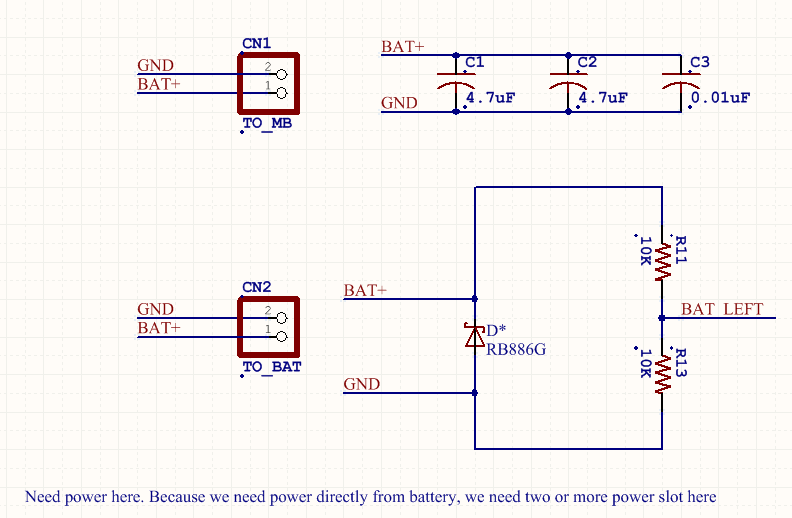
\includegraphics[width=0.9\textwidth]{power_bridge.png}
    \caption{\label{fig:power_bridge}Power Bridge and coupling}
    \end{figure} 

 



  \subsubsection{On-board power}
    \label{power block}
    
    \begin{figure}[ht]
    \centering
    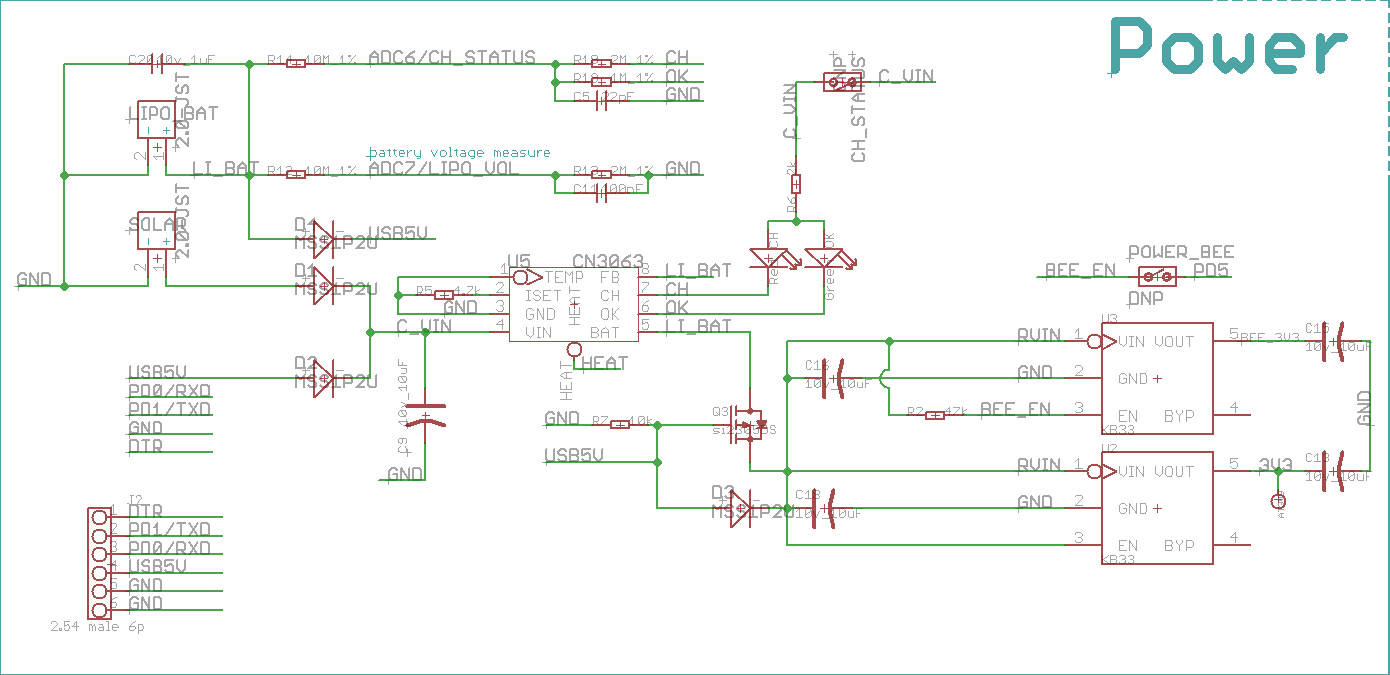
\includegraphics[width=0.9\textwidth]{3v3power_circuit.png}
    \caption{\label{fig:3v3power_circuit}On board power regulator}
    \end{figure}  
    Seeeduino Stalker v2.3 has regulator to regulate external power supply to 3.3V standard, and all GPIO output is in 3.3V standard. 


    \begin{figure}[H]
    \centering
    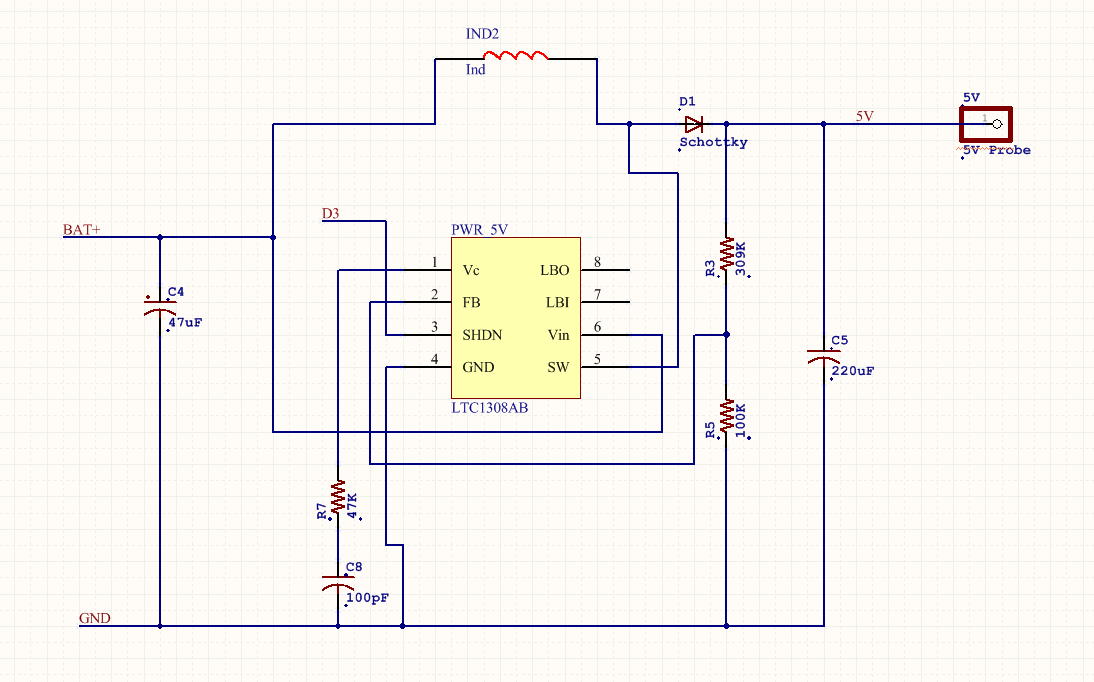
\includegraphics[width=0.9\textwidth]{power_circuit.png}
    \caption{\label{fig:power_circuit}On board power boost circuit}
    \end{figure}
    In order to power on 5V standard peripheral devices, there is voltage boost regulator on the functionality board to boost battery voltage to 5V standard. This power boost chip's SHUTDOWN pin is controlled\footnotemark by D5 pin on the controller board. \\
    
    \footnotetext{\textbf{$\bigstar$Known bug} Due to the design of voltage boost chip, when D5 pin is LOW, this boost circuit still gives out 3.2V output} 

  
  \subsection{RTC}
    DS3231 chip is Extremely accurate $I^{2}C-intergrated$ RTC from Maximintegrated company. This data-logger has on-board DS3231 chip with backup button battery to keep timing, and wake up in period of time, which is excellent for extending battery life.  \\
    According to the offical application document from Seeeduino Wiki page, using RTC to wake up controller and put it into sleep mode can dramatically lower the power comsumption.
    \begin{framed}
            \begin{itemize}
            \item The current consumption at sleep mode is 95.82 uA at 3.3V (i.e 316.206 uW power consumption). Please note, that the SD Card VCC is still powered in this demo. 
            \item The current consumption at active mode peak is 22.43 mA @ 3.3V (i.e 74.019 mW power consumption)
            \end{itemize}
    \end{framed}


  \subsection{$I^{2}C$ Design}
    \label{i2c Design}
    $I^{2}C$ is important port in this data-logger, because devices inlcuding external ADC and precise temperature sensors are depending on $I^{2}C$ to send data to the controller. \\
    
    \subsubsection{$I^{2}C$ Port}
    $I^{2}C$ Port on Seeeduino Stalker is signed to Analog pins area, a different from Arduino Uno.
    
    \begin{figure}[H]
    \centering
    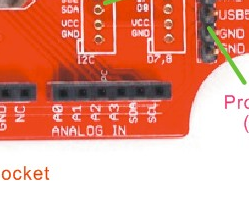
\includegraphics[width=0.9\textwidth]{i2cPort.png}
    \caption{\label{fig:i2c Port}$I^{2}C$ port position on the Controller board}
    \end{figure}

    \subsubsection{$I^{2}C$ Level shifting}
    \begin{figure}[H]
    \centering
    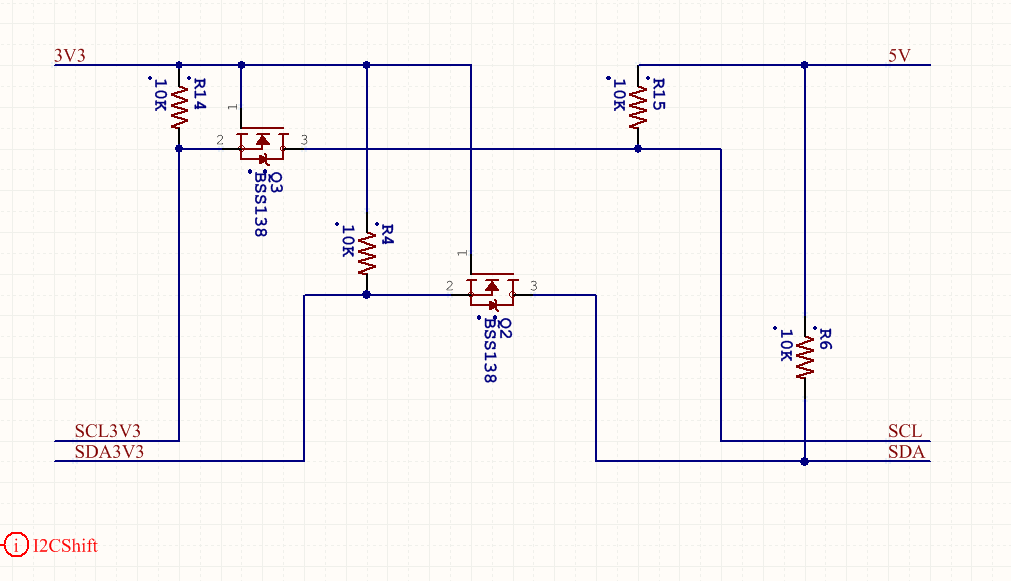
\includegraphics[width=0.9\textwidth]{i2clevelshift.png}
    \caption{\label{fig:i2c Level shift}$I^{2}C$ Level Shift circuit}
    \end{figure}
    Because all the external devices are working under 5V standard, so there is 2-way $I^{2}C$ level shifting circuit\footnotemark on the functionality board to convert 5V to 3.3V, verse versa.

    \footnotetext{Thanks to the application document \textit{Bi-directional level shifter for
I2C-bus and other systems} from PHILIPS}

    \subsection{Enhanced ADC}

    \begin{figure}[H]
    \centering
    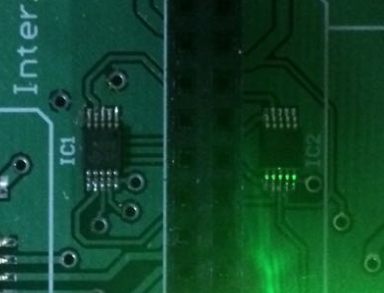
\includegraphics[width=0.9\textwidth]{adcPosition.png}
    \caption{\label{fig:i2c adcPosition}ADS1115 chip position on the functionality board}
    \end{figure}

    In order to eliminate noise, ADC chips are located as close as possible to the center connector.

    Two ADS1115 16-bit high precision ADC chips from TI are used on the functionality board. These ADC circuits use $I^{2}C$ protocal and give reliable rail-to-rail measuring ability to the data-logger. According to the design, 8 ADC ports are exposured to the outside world. User can either use them as 8 single-ended ADC inputs or 4 pair of differential ADC inputs.

    \begin{figure}[H]
    \centering
    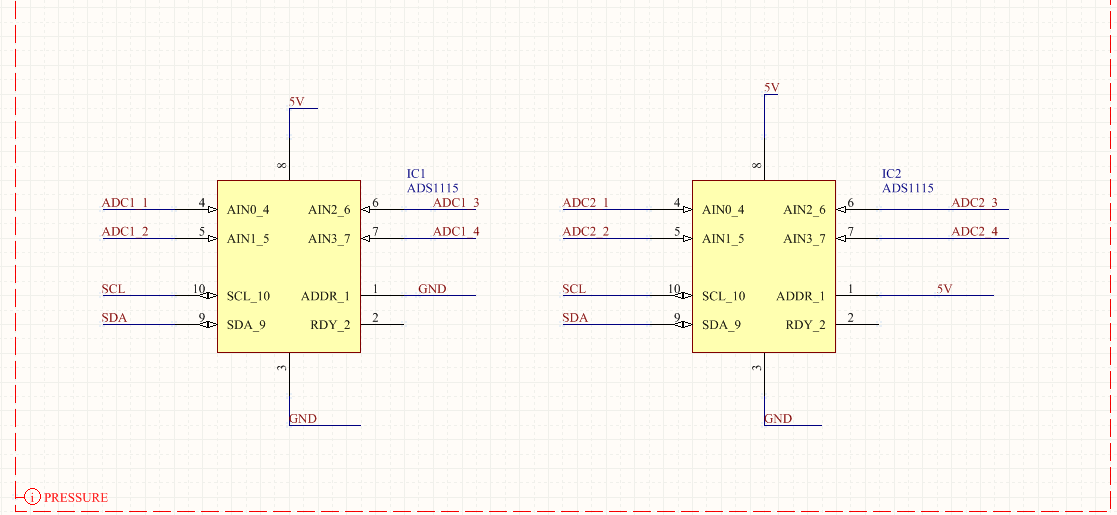
\includegraphics[width=0.9\textwidth]{adcSch.png}
    \caption{\label{fig:i2c schematic}ADS1115 chip schematic}
    \end{figure}

    Two ADS1115 chips are configured with two $I^{2}C$ address. No.1 chip is 0x48, and No.2 chip is 0x49.
    Refering to \hyperref[absValue]{\textbf{\textit{Absolute Value}}} for more information.



  \subsection{Read-Only Port}
    \label{read-only Design}
    \begin{figure}[H]
    \centering
    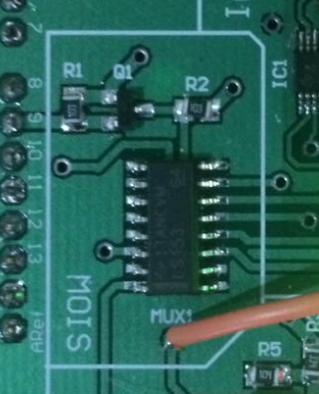
\includegraphics[width=0.9\textwidth]{mosPosition.png}
    \caption{\label{fig:moisture sensor position}Read-Only port position on the board}
    \end{figure}
    Read Only port is implemented by a SoftSerial port on the controller and a 4-to-1 74x153 MUX chip with level shifter circuit, located on the side of functionality board.


    \begin{figure}[H]
    \centering
    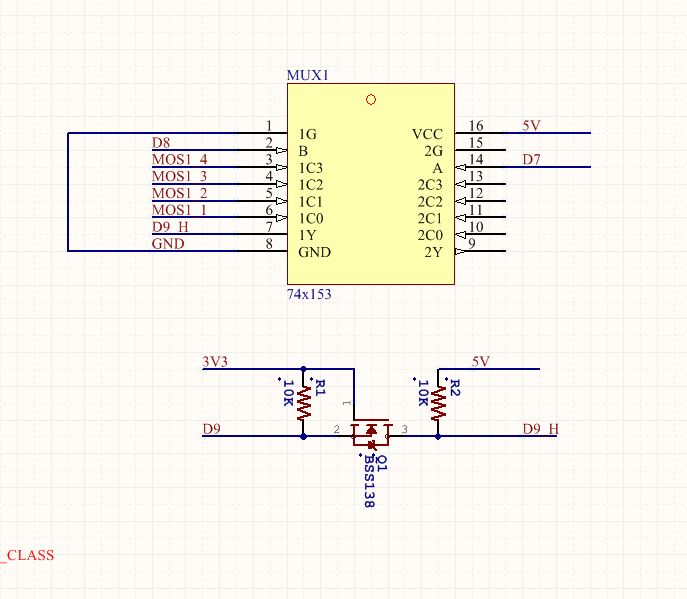
\includegraphics[width=0.9\textwidth]{mosSch.png}
    \caption{\label{fig:moisture sensor schematic}Read-Only port schematic}
    \end{figure}
    The moisture sensor, Decagon 5TE sensor uses 1-wire communication protocal which is compatible to Serial/UART port, so controller is able to read up to four 5TE sensors or other read-only sensors. \\
    MUX has two select pins, which are D7 and D8. The output pin of group 1 is D9(5V), which will be converted to 3.3V standard, and this MUX is always enabled. The second group of 4-to-1 MUX on this 74x153 chip is not used.




  \subsection{Dimensions}
    \begin{figure}[H]
    \centering
    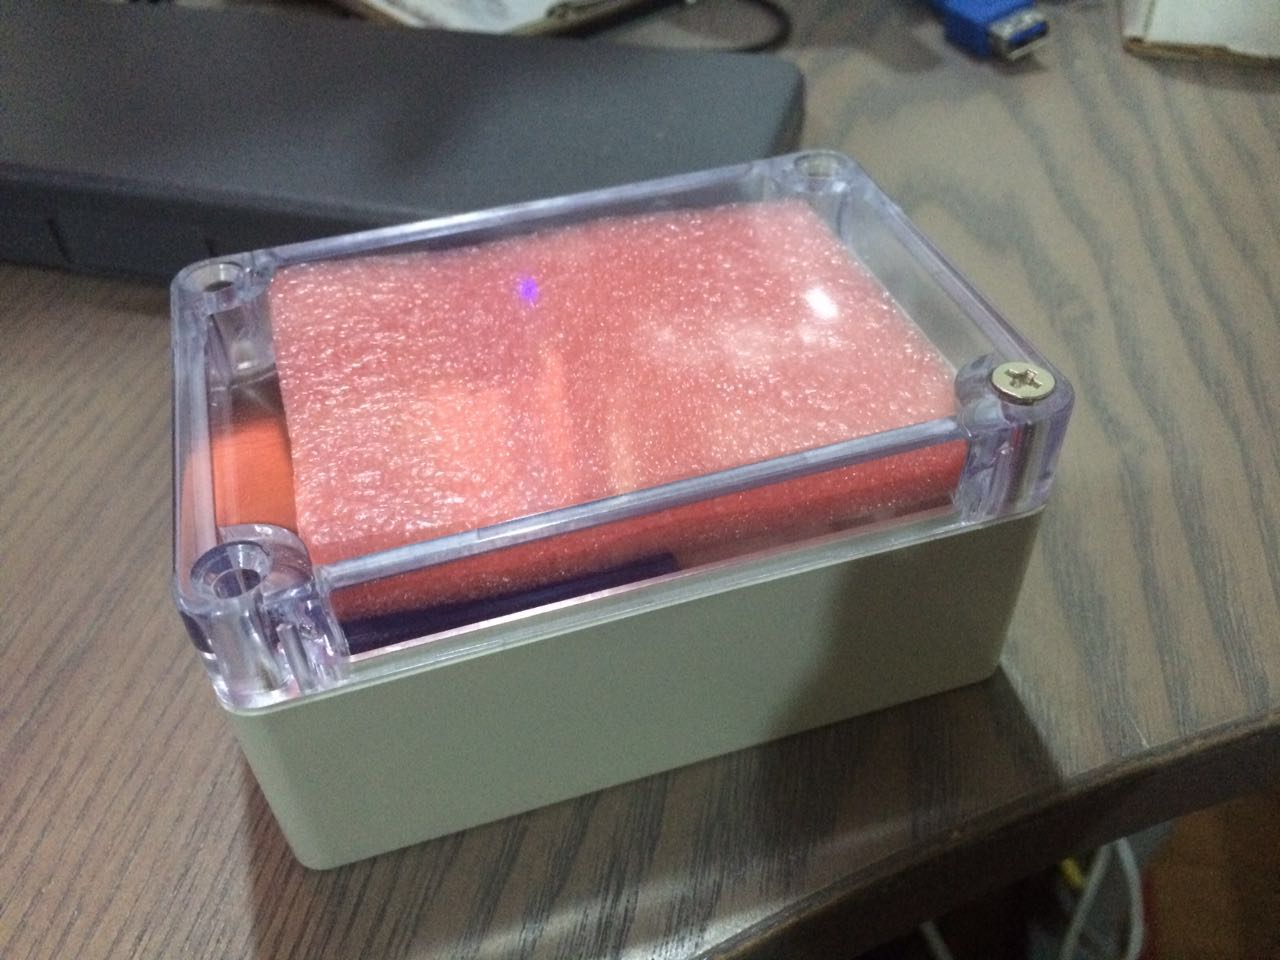
\includegraphics[width=0.9\textwidth]{box.jpg}
    \caption{\label{fig:water-resistant box}Water-resistant box}
    \end{figure}
    All the parts, excluded connection wires can fit in a water-resistant box, which has dimension as 3.95in(100mm) X 2.68in(68mm) X 1.96in(50mm).

    \begin{figure}[H]
    \centering
    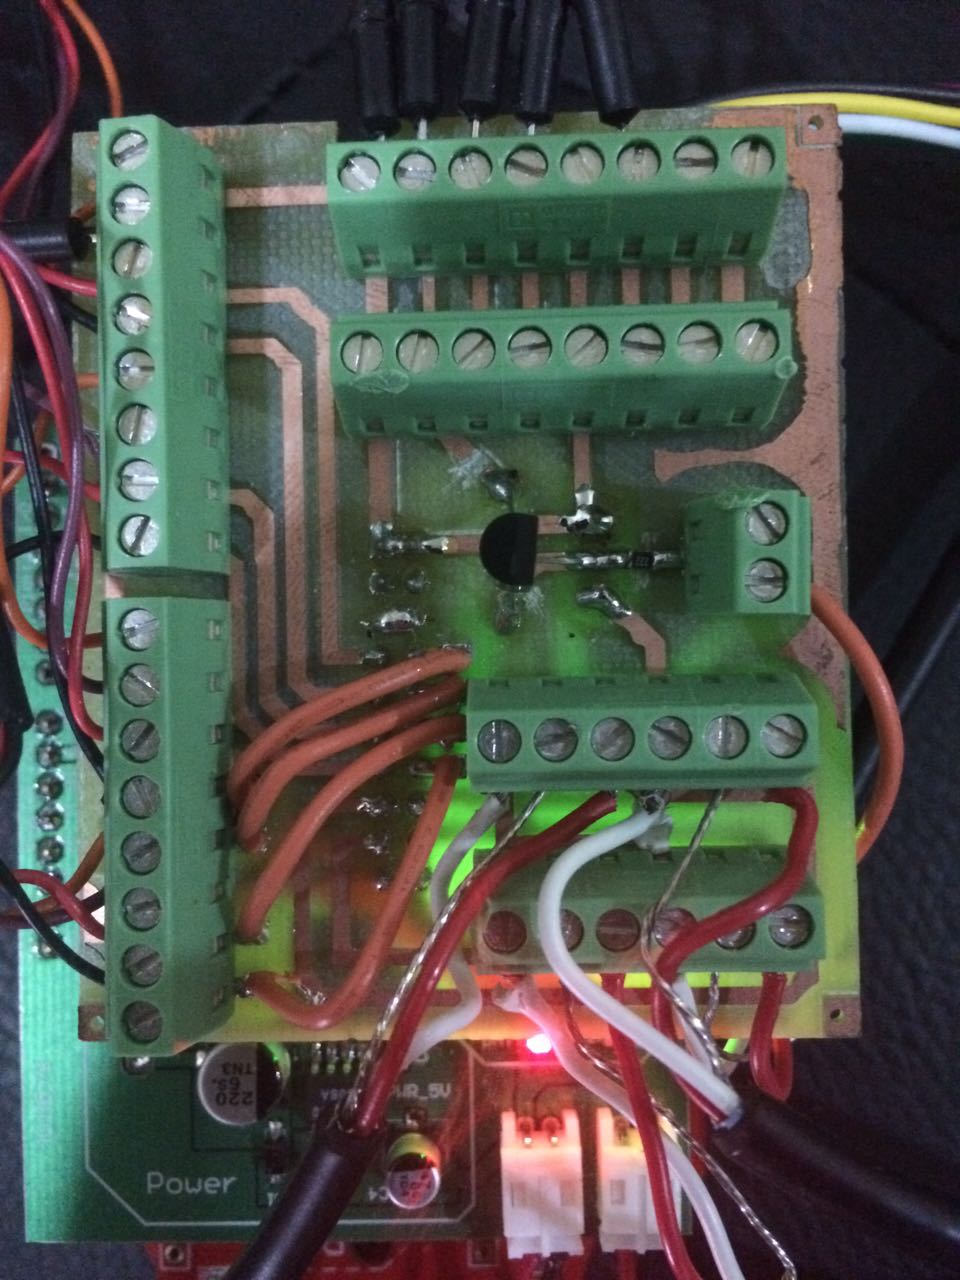
\includegraphics[width=0.9\textwidth]{con_board_top.jpg}
    \caption{\label{fig:Con Board}Connectivity Board Top view}
    \end{figure}
    All the parts, excluded connection wires can fit in a water-resistant box, which has dimension as 2.5in(63.5mm) X 2.1in(53.34mm) X 0.4in(10mm).

  
         

\newpage
\section{Software Design}


    \subsection{Overall strucutre}
    All the components in this robot are written in C and optimized for power-saving consideration.   \\
    The following libraries are in use: \\
    \begin{itemize}
        \item <avr/sleep.h>
        \item <avr/power.h>
        \item <EEPROM.h>
        \item <SdFat.h>
        \item <stdio.h>
        \item <Wire.h>
        \item <SoftwareSerial.h>
        \item <Adafruit\_ADS1015.h>
        \item <DS3231.h>
        \item <Adafruit\_MCP9808.h>
    \end{itemize}
       And no customize library in use, so the firmware is better for general purpose usage.

% \newpage
\section{Future Work}
\subsection{Wireless}
Now the data-logger is in its release 1.0 version, and I am already started working on the 2.0 version, which is data-logger local network that has a coordinator to collect log files everyday them send them to the cloud.



\begin{appendices}

    \section{PCB Design}
        \subsection{Functionality board}
           \begin{figure}[H]
            \centering
            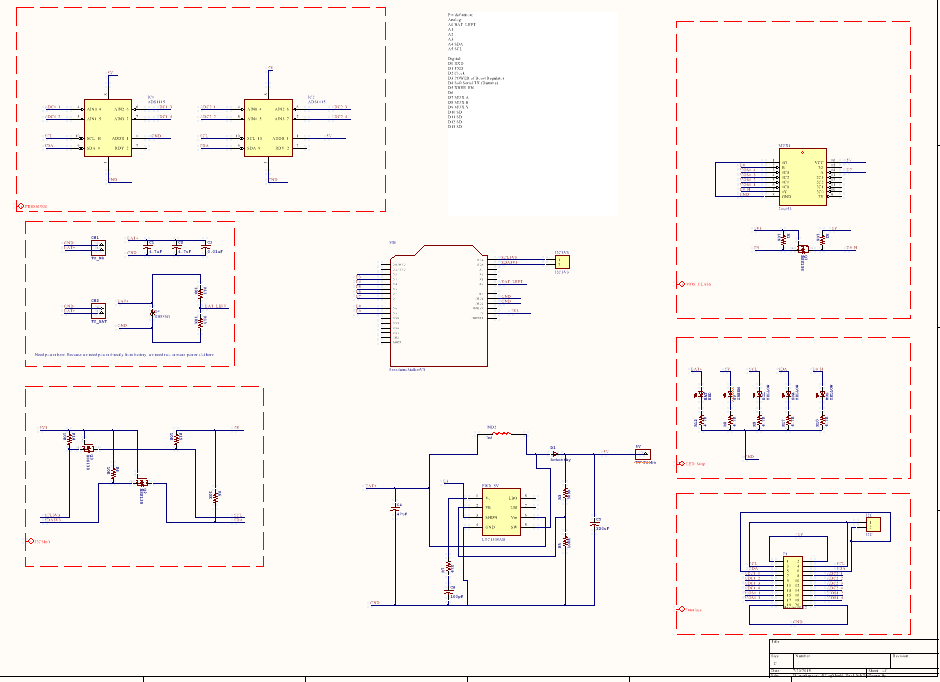
\includegraphics[width=0.2\textwidth]{funcSch.png}
            \caption{\label{fig:func_sch}Functionality board PCB schematic}
            \end{figure}

            \begin{figure}[H]
            \centering
            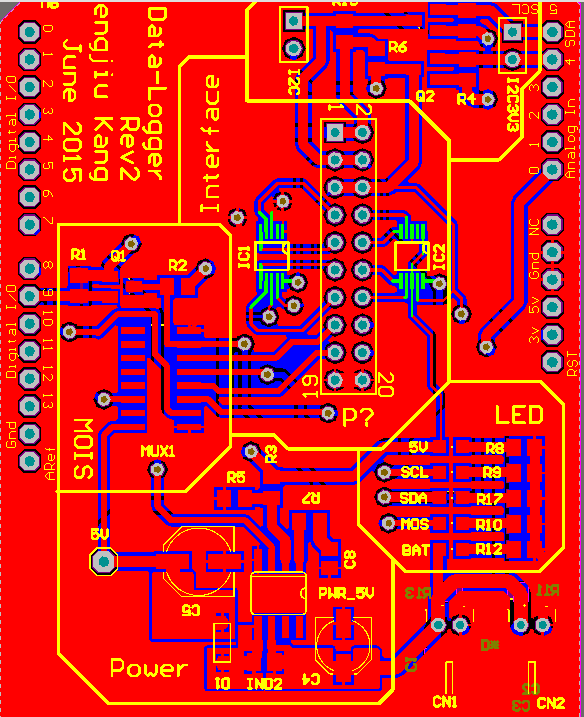
\includegraphics[width=0.2\textwidth]{funcBrd.png}
            \caption{\label{fig:func_brd}Functionality board PCB Layout}
            \end{figure}

        \subsection{Connectivity board}
            \begin{figure}[H]
            \centering
            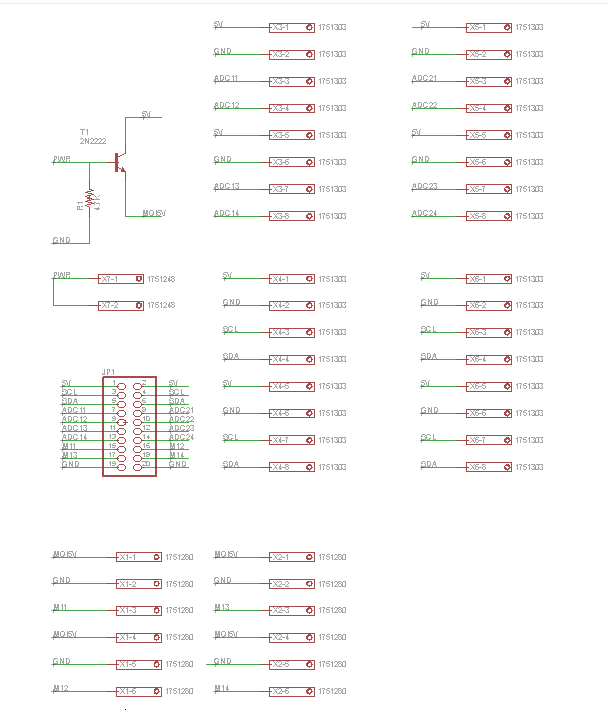
\includegraphics[width=0.2\textwidth]{conSch.png}
            \caption{\label{fig:con_sch}Connectivity board PCB schematic}
            \end{figure}

            \begin{figure}[H]
            \centering
            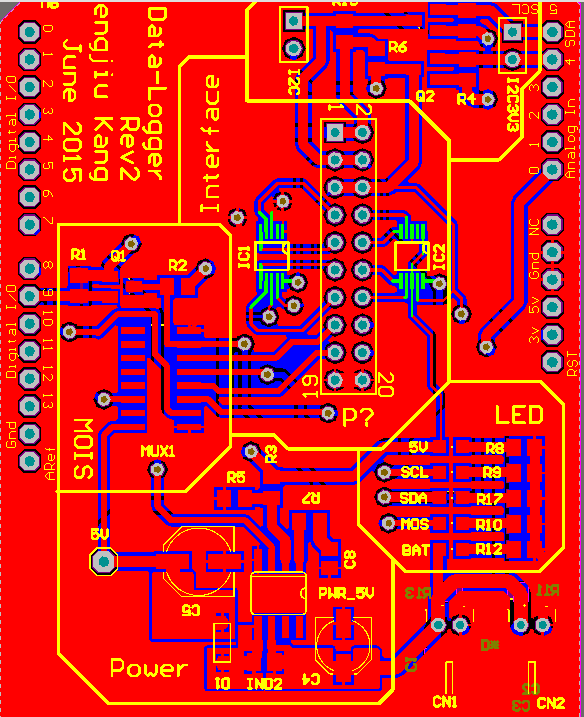
\includegraphics[width=0.2\textwidth]{funcBrd.png}
            \caption{\label{fig:con_brd}Connectivity board PCB Layout}
            \end{figure}

    \section{BOM}
    Due to limited space, please check individual BOM file.

    \section{Source code}
        \subsection{Applications}
            \label{source:applications}
            \subsubsection{Main on Beaglebone Black}
                 \lstinputlisting[language=C++]{src/ver400.ino}

\end{appendices}


% \todo {parts following are for referencing, because Im not familiar with latex}
% \subsection{Tables and Figures}

% Use the table and tabular commands for basic tables --- see Table~\ref{tab:widgets}, for example. You can upload a figure (JPEG, PNG or PDF) using the files menu. To include it in your document, use the includegraphics command as in the code for Figure~\ref{fig:frog} below.

% % Commands to include a figure:
% \begin{figure}
% \centering
% \includegraphics[width=0.5\textwidth]{frog.jpg}
% \caption{\label{fig:frog}This is a figure caption.}
% \end{figure}

% \begin{table}
% \centering
% \begin{tabular}{l|r}
% Item & Quantity \\\hline
% Widgets & 42 \\
% Gadgets & 13
% \end{tabular}
% \caption{\label{tab:widgets}An example table.}
% \end{table}

% \subsection{Mathematics}

% \LaTeX{} is great at typesetting mathematics. Let $X_1, X_2, \ldots, X_n$ be a sequence of independent and identically distributed random variables with $\text{E}[X_i] = \mu$ and $\text{Var}[X_i] = \sigma^2 < \infty$, and let
% $$S_n = \frac{X_1 + X_2 + \cdots + X_n}{n}
%       = \frac{1}{n}\sum_{i}^{n} X_i$$
% denote their mean. Then as $n$ approaches infinity, the random variables $\sqrt{n}(S_n - \mu)$ converge in distribution to a normal $\mathcal{N}(0, \sigma^2)$.

% \subsection{Lists}

% You can make lists with automatic numbering \dots

% \begin{enumerate}
% \item Like this,
% \item and like this.
% \end{enumerate}
% \dots or bullet points \dots
% \begin{itemize}
% \item Like this,
% \item and like this.
% \end{itemize}

% We hope you find write\LaTeX\ useful, and please let us know if you have any feedback using the help menu above.

\end{document}